\documentclass{article}
\usepackage[utf8]{inputenc}
\usepackage{mathrsfs}
\usepackage{tikz}
\usepackage{amssymb}
\usepackage{amsthm}
\usepackage{graphicx} % Required for inserting images
\usepackage{amsmath}
\usepackage{MnSymbol}
\usepackage{geometry}
\usepackage{physics}
\usepackage{enumerate}
\allowdisplaybreaks
\newcommand\numeq[1]%
  {\stackrel{\scriptscriptstyle(\mkern-1.5mu#1\mkern-1.5mu)}{=}}
\newcommand\numleq[1]
  {\stackrel{\scriptscriptstyle(\mkern-1.5mu#1\mkern-1.5mu)}{\leq}}
\newcommand\numgeq[1]
  {\stackrel{\scriptscriptstyle(\mkern-1.5mu#1\mkern-1.5mu)}{\geq}}

\newtheorem{definition}{Definition}[section]
\newtheorem{theorem}{Theorem}[section]
\newtheorem{remark}{Remark}[section]
\newtheorem{example}{Example}[section]



\title{Math 132H Homework 2}
\author{Tom Slavonia}
\date{\today}

\begin{document}
\maketitle

\section*{24.}
\begin{proof}
Assume we are given $[a, b] \subset \mathbb{R}$, an interval, $z: [a, b] \xrightarrow[t \mapsto z(t)]{} \mathbb{C}$. We also then have the parametrization $z^-(t) = z(b + a - t)$, which is the reverse orientation of $z(t)$, and we have the bijection $t(s) = (b + a - s)$. Therefore, we have that $z$ and $z^-$ are equivalent parametrizations. Hence, we have that 
\begin{align*}
  \int_{\gamma} f(z) \mathrm{d}z &\numeq{a} \int_a^b f(z(t)) z^{\prime}(t) \mathrm{d}t \\
  &\numeq{b} \int_b^a f(z^-(s))z^{- \prime}(s) \mathrm{d}s \\
  &\numeq{c} -\int_a^bf(z^-(s))z^{-\prime}(s) \mathrm{d}s \\
  &\numeq{d} - \int_{\gamma^-}f(z) \mathrm{d}z. \\ 
\end{align*}
Steps $(a) - (d)$ are justified below:
\begin{enumerate}[\indent(a)]
  \item Equivalent definition of the integral over $\gamma$
  \item Using that $z(t(s))$ and $z^-(s)$ are equivalent parametrizations
  \item Swapping bounds of integration requires us to multiply by negative one
  \item Reverse of justification $(a)$.
\end{enumerate} 



\end{proof}

\section*{25.}
\subsection*{a.}
\begin{proof}
Let $\gamma$ be any circle with counterclockwise orientation centered at the origin. Here we have that $z(t) = re^{it} + c$ for $|c| < r$. We begin by integrating when $n \neq 1$:
\begin{align*}
  \int_{\gamma}z^n \mathrm{d}z &= \int_0^{2\pi}z(t)^nz'(t)\mathrm{d}t\\
  &= \int_0^{2\pi} r^ne^{itn}ire^{it} \mathrm{d}t\\
  &= r^{n + 1}i\int_0^{2\pi}e^{it(n + 1)} \mathrm{d}t \\
  &\numeq{a} r^{n+1}i \int_0^{2 \pi} \left(\frac{1}{i(n + 1)}e^{it(n + 1)} \right)^{\prime} \mathrm{d}t\\
  &\numeq{b} r^{n+1}i \int_0^{2 \pi} \frac{d}{dt}\left(-\frac{i}{n + 1}e^{it(n + 1)} \right)\mathrm{d}t \\
  &\numeq{c} r^{n+1}i \left(-\frac{i}{n + 1}e^{i2\pi(n + 1)} + \frac{i}{n + 1}e^{i 0 (n + 1)} \right)\\
  &= r^{n+1}i \left(-\frac{i}{n + 1}(\cos(2\pi(n + 1)) + i \sin(2\pi(n + 1))) + \frac{i}{n + 1}\cdot 1 \right)\\
  &= r^{n+1}i\left(-\frac{i}{n + 1} + \frac{i}{n + 1} \right) \\
  &= 0.
\end{align*}
%Let $\gamma$ be any circle with counterclockwise orientation centered at the origin. Here we have that $z(t) = re^{it}$. We begin by integrating when $n \neq 1$, but we notice that in this case $z^n$ has a primitive, $\frac{1}{n + 1}z^{n + 1}$ and thus we have that since $\gamma$ is in an open disc and 
The steps $(a)-(c)$ are justified:
\begin{enumerate}[\indent(a)]
  \item $\frac{1}{i(n + 1)}e^{it(n + 1)}$ is holomorphic on the set with derivative $e^{it(n + 1)}$
  \item $\frac{1}{i} = \frac{i}{i^2} = -i$
  \item Fundamental theorem of calculus.
\end{enumerate}
In the case where $n = -1$ the solution differs: 
\begin{align*}
  \int_{\gamma}z^{-1} \mathrm{d}z &= \int_0^{2\pi} z(t)^{-1} z'(t) \mathrm{d}t \\
  &= \int_0^{2 \pi} r^{-1}e^{-it}ire^{it} \mathrm{d}t \\
  &= i\int_0^{2 \pi} e^{-it + it}\mathrm{d}t \\
  &= i\int_0^{2 \pi} \mathrm{d}t \\
  &= i(2 \pi - 0) \\
  &= 2\pi  i.
\end{align*}
\end{proof}

\subsection*{b.}
\begin{proof}
  Focusing on when $\gamma$, a circle, does not contain the origin, therefore $z(t) = re^{it} + c$ for $|c| > r$ is a valid parametrization of $\gamma$. Note that $z'(t) = rie^{it}$. For $n \neq -1$, we have that $f(z) = z^n$ has a primitive, namely $\frac{1}{n + 1}z^{n + 1}$ on $\gamma$, and thus by a corollary in the book, since a circle $\gamma$ is a closed curve, and we can enclose that closed curve inside a larger open disc, we have that, by Cauchy's theorem
  \[
  \int_{\gamma} z^n \mathrm{d}z = 0. 
  \] 
  %For the case where $n = -1$, since we don't contain the origin, we can create the picture below and use Cauchy's theorem as well as the existence of local primitives to get that 
  %\[
  %\int_{\gamma} z^{-1} \mathrm{d}z = 0.   
  %\]


\end{proof}

\subsection*{c.}
\begin{proof}
  Suppose $|a| < r < |b|$, and $\gamma$ is a circle centered around the origin with radius $r$ and oriented in the positive direction. The integral 
  \begin{align*}
    \int_{\gamma}\frac{1}{(z - a)(z - b)} \mathrm{d}z &\numeq{a}\int_{\gamma}\frac{1}{a - b} \left(\frac{1}{z - a} - \frac{1}{z - b} \right) \mathrm{d}z \\
    &= \frac{1}{a - b}\left(\int_{\gamma}\frac{1}{z - a} \mathrm{d}z - \int_{\gamma}\frac{1}{z-b} \mathrm{d}z \right) \\
    &= \frac{2 \pi i}{a - b}
  \end{align*}
  this is true as we can create the picture below and use Cauchy's theorem and the local existence of primitives. We also have that $|a| < r < |b|$, so the integral $\int_{\gamma}\frac{1}{z - a} \mathrm{d}z$ is inside $\gamma$ and the integral $\int_{\gamma}\frac{1}{z - b} \mathrm{d}z$ is outside of $\gamma$, so we can apply the earlier parts of the problem to solve. We can use partial fraction decomposition to break apart the integral like so:
  \[
    \frac{1}{(z - a)(z - b)} = \frac{A}{z - a} + \frac{B}{z - b}  
    \]
    \[
    \Rightarrow 1 = A(z - b) + B(z - a)  
    \]
    solving for $A$ and $B$ we get
    \[
    \frac{1}{a - b} = A = B.  
    \]
  \begin{center}
    \tikzset{every picture/.style={line width=0.75pt}} %set default line width to 0.75pt        
    
    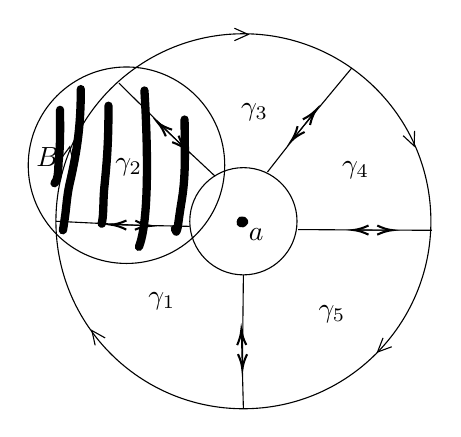
\begin{tikzpicture}[x=0.5pt,y=0.5pt,yscale=-1,xscale=1]
    %uncomment if require: \path (0,300); %set diagram left start at 0, and has height of 300
    
    %Shape: Circle [id:dp461238716807183] 
    \draw   (198,148.5) .. controls (198,73.67) and (258.67,13) .. (333.5,13) .. controls (408.33,13) and (469,73.67) .. (469,148.5) .. controls (469,223.33) and (408.33,284) .. (333.5,284) .. controls (258.67,284) and (198,223.33) .. (198,148.5) -- cycle ;
    %Shape: Circle [id:dp08084106343870379] 
    \draw   (294.75,148.5) .. controls (294.75,127.1) and (312.1,109.75) .. (333.5,109.75) .. controls (354.9,109.75) and (372.25,127.1) .. (372.25,148.5) .. controls (372.25,169.9) and (354.9,187.25) .. (333.5,187.25) .. controls (312.1,187.25) and (294.75,169.9) .. (294.75,148.5) -- cycle ;
    %Shape: Free Drawing [id:dp7381659893993409] 
    \draw  [line width=3] [line join = round][line cap = round] (333,150) .. controls (333,150) and (333,150) .. (333,150) .. controls (333.53,148.93) and (332.53,146.93) .. (332,148) .. controls (330.23,151.53) and (333.74,149.26) .. (334,149) .. controls (334.33,148.67) and (333.47,148) .. (333,148) ;
    \draw   (226.38,238.2) -- (224.01,227.49) -- (233.6,232.82) ;
    \draw   (201.53,103.42) -- (208.07,94.62) -- (210.32,105.35) ;
    %Straight Lines [id:da277193417876471] 
    \draw    (333.5,284) -- (332.05,229) ;
    \draw [shift={(332,227)}, rotate = 88.49] [color={rgb, 255:red, 0; green, 0; blue, 0 }  ][line width=0.75]    (10.93,-3.29) .. controls (6.95,-1.4) and (3.31,-0.3) .. (0,0) .. controls (3.31,0.3) and (6.95,1.4) .. (10.93,3.29)   ;
    %Straight Lines [id:da6479299525313575] 
    \draw    (333.5,187.25) -- (332.77,253.5) ;
    \draw [shift={(332.75,255.5)}, rotate = 270.63] [color={rgb, 255:red, 0; green, 0; blue, 0 }  ][line width=0.75]    (10.93,-3.29) .. controls (6.95,-1.4) and (3.31,-0.3) .. (0,0) .. controls (3.31,0.3) and (6.95,1.4) .. (10.93,3.29)   ;
    %Straight Lines [id:da25834140326970534] 
    \draw    (294.68,152.18) -- (240,151.04) ;
    \draw [shift={(238,151)}, rotate = 1.19] [color={rgb, 255:red, 0; green, 0; blue, 0 }  ][line width=0.75]    (10.93,-3.29) .. controls (6.95,-1.4) and (3.31,-0.3) .. (0,0) .. controls (3.31,0.3) and (6.95,1.4) .. (10.93,3.29)   ;
    %Straight Lines [id:da7508484532716964] 
    \draw    (198,148.5) -- (264.17,151.75) ;
    \draw [shift={(266.17,151.85)}, rotate = 182.81] [color={rgb, 255:red, 0; green, 0; blue, 0 }  ][line width=0.75]    (10.93,-3.29) .. controls (6.95,-1.4) and (3.31,-0.3) .. (0,0) .. controls (3.31,0.3) and (6.95,1.4) .. (10.93,3.29)   ;
    %Straight Lines [id:da7410402747275302] 
    \draw    (313.1,115.98) -- (273.15,78.63) ;
    \draw [shift={(271.69,77.26)}, rotate = 43.07] [color={rgb, 255:red, 0; green, 0; blue, 0 }  ][line width=0.75]    (10.93,-3.29) .. controls (6.95,-1.4) and (3.31,-0.3) .. (0,0) .. controls (3.31,0.3) and (6.95,1.4) .. (10.93,3.29)   ;
    %Straight Lines [id:da6673936530245965] 
    \draw    (243.58,48.7) -- (290.68,95.29) ;
    \draw [shift={(292.1,96.7)}, rotate = 224.69] [color={rgb, 255:red, 0; green, 0; blue, 0 }  ][line width=0.75]    (10.93,-3.29) .. controls (6.95,-1.4) and (3.31,-0.3) .. (0,0) .. controls (3.31,0.3) and (6.95,1.4) .. (10.93,3.29)   ;
    %Straight Lines [id:da7763481211665251] 
    \draw    (350.88,112.92) -- (384.58,69.85) ;
    \draw [shift={(385.81,68.27)}, rotate = 128.04] [color={rgb, 255:red, 0; green, 0; blue, 0 }  ][line width=0.75]    (10.93,-3.29) .. controls (6.95,-1.4) and (3.31,-0.3) .. (0,0) .. controls (3.31,0.3) and (6.95,1.4) .. (10.93,3.29)   ;
    %Straight Lines [id:da474462409183386] 
    \draw    (411.8,37.76) -- (369.52,88.77) ;
    \draw [shift={(368.24,90.31)}, rotate = 309.66] [color={rgb, 255:red, 0; green, 0; blue, 0 }  ][line width=0.75]    (10.93,-3.29) .. controls (6.95,-1.4) and (3.31,-0.3) .. (0,0) .. controls (3.31,0.3) and (6.95,1.4) .. (10.93,3.29)   ;
    %Straight Lines [id:da8057652971094238] 
    \draw    (469.68,155) -- (415,154.85) ;
    \draw [shift={(413,154.84)}, rotate = 0.16] [color={rgb, 255:red, 0; green, 0; blue, 0 }  ][line width=0.75]    (10.93,-3.29) .. controls (6.95,-1.4) and (3.31,-0.3) .. (0,0) .. controls (3.31,0.3) and (6.95,1.4) .. (10.93,3.29)   ;
    %Straight Lines [id:da5850403826169577] 
    \draw    (373,154.5) -- (439.17,154.94) ;
    \draw [shift={(441.17,154.95)}, rotate = 180.38] [color={rgb, 255:red, 0; green, 0; blue, 0 }  ][line width=0.75]    (10.93,-3.29) .. controls (6.95,-1.4) and (3.31,-0.3) .. (0,0) .. controls (3.31,0.3) and (6.95,1.4) .. (10.93,3.29)   ;
    \draw   (440.72,239.21) -- (430.43,243) -- (434.42,232.79) ;
    \draw   (457.21,83.15) -- (456.94,94.11) -- (448.91,86.64) ;
    \draw   (327,9) -- (337,13.5) -- (327,18) ;
    %Shape: Circle [id:dp6266915097079111] 
    \draw   (178,108) .. controls (178,68.79) and (209.79,37) .. (249,37) .. controls (288.21,37) and (320,68.79) .. (320,108) .. controls (320,147.21) and (288.21,179) .. (249,179) .. controls (209.79,179) and (178,147.21) .. (178,108) -- cycle ;
    %Shape: Free Drawing [id:dp3182375546543479] 
    \draw  [line width=3] [line join = round][line cap = round] (216,53) .. controls (216,78.96) and (213.5,97.15) .. (208,121) .. controls (206.44,127.77) and (205.78,134.95) .. (205,142) .. controls (204.69,144.78) and (203,156.16) .. (203,155) ;
    %Shape: Free Drawing [id:dp8543299302897445] 
    \draw  [line width=3] [line join = round][line cap = round] (201,68) .. controls (201,80.34) and (201.36,92.74) .. (200,105) .. controls (199.54,109.11) and (200.19,117.81) .. (197,121) ;
    %Shape: Free Drawing [id:dp12436087987725619] 
    \draw  [line width=3] [line join = round][line cap = round] (262,54) .. controls (262,56.43) and (268.05,141.86) .. (258,167) ;
    %Shape: Free Drawing [id:dp7119451536286852] 
    \draw  [line width=3] [line join = round][line cap = round] (236,65) .. controls (236,90.14) and (235.13,102.7) .. (233,124) .. controls (232.33,130.66) and (232.42,137.31) .. (232,144) .. controls (231.87,146.02) and (231,152.03) .. (231,150) ;
    %Shape: Free Drawing [id:dp09765979791505885] 
    \draw  [line width=3] [line join = round][line cap = round] (291,75) .. controls (291,94.34) and (292.18,113.92) .. (289,133) .. controls (287.87,139.8) and (286.97,146.22) .. (286,153) .. controls (285.85,154.04) and (285,156) .. (285,156) .. controls (285,156) and (284.2,154.2) .. (284,154) ;
    
    % Text Node
    \draw (335.5,151.9) node [anchor=north west][inner sep=0.75pt]    {$a$};
    % Text Node
    \draw (263,198.4) node [anchor=north west][inner sep=0.75pt]    {$\gamma _{1}$};
    % Text Node
    \draw (386,207.4) node [anchor=north west][inner sep=0.75pt]    {$\gamma _{5}$};
    % Text Node
    \draw (403,103.4) node [anchor=north west][inner sep=0.75pt]    {$\gamma _{4}$};
    % Text Node
    \draw (330,61.4) node [anchor=north west][inner sep=0.75pt]    {$\gamma _{3}$};
    % Text Node
    \draw (239,101.4) node [anchor=north west][inner sep=0.75pt]    {$\gamma _{2}$};
    % Text Node
    \draw (182,93.4) node [anchor=north west][inner sep=0.75pt]    {$B$};
    
    
    \end{tikzpicture}
    \end{center} 
  %with steps $(a) - (b)$ justified:
  %\begin{enumerate}[\indent(a)]
   %\item using partial fraction decomposition, we see
    %\[
    %\frac{1}{(z - a)(z - b)} = \frac{A}{z - a} + \frac{B}{z - b}  
    %\]
    %\[
    %\Rightarrow 1 = A(z - b) + B(z - a)  
    %\]
    %solving for $A$ and $B$ we get
    %\[
    %\frac{1}{a - b} = A = B  
    %\]
    %\item Because $|a| < r$ and $|b| > r$ the integral \[\int_{\gamma}\frac{1}{z - a} \mathrm{d}z\] contains the origin so that we can apply the first part of the problem, and \[
    %\int_{\gamma}\frac{1}{z - b}\mathrm{d}z  
    %\]
    %does not contain the origin, so we can apply the second part of the problem. 
  %\end{enumerate}

\end{proof}




\section*{26.}
\begin{proof}
  Suppose $F(z)$ and $G(z)$ are primitives of $f(z)$. We then have that 
  \[
  0 = f(z) - f(z) = F'(z) - G'(z) = (F(z) - G(z))'  
  \]
  by the linearity of the derivative. 
\end{proof}

\section*{1.}
\subsection*{a.}
\begin{proof}
  Take $f(z) = e^{-z^2}$. Using Cauchy's theorem, because if $\gamma$ is the entire path in the figure, then it is closed and can be surrounded by an open disc, and since $f$ is holomorphic, we have
  \[
  0 = \int_{\gamma}f(z) \mathrm{d}z = \int_{\gamma}e^{-z^2} \mathrm{d}z.
  \]
  Let $\gamma_1$, $\gamma_2$, $\gamma_3$ be curves shown in the figure below

\begin{center}
\tikzset{every picture/.style={line width=0.75pt}} %set default line width to 0.75pt        

\begin{tikzpicture}[x=0.75pt,y=0.75pt,yscale=-1,xscale=1]
%uncomment if require: \path (0,300); %set diagram left start at 0, and has height of 300

%Shape: Axis 2D [id:dp7523876561837348] 
\draw  (236,225.6) -- (439,225.6)(256.3,51) -- (256.3,245) (432,220.6) -- (439,225.6) -- (432,230.6) (251.3,58) -- (256.3,51) -- (261.3,58)  ;
%Shape: Arc [id:dp5531989103320447] 
\draw  [draw opacity=0] (351.34,143.51) .. controls (377.42,163.05) and (392.33,193.04) .. (393.92,224.52) -- (285.23,232.56) -- cycle ; \draw   (351.34,143.51) .. controls (377.42,163.05) and (392.33,193.04) .. (393.92,224.52) ;  
%Straight Lines [id:da06183978011979585] 
\draw    (351.34,143.51) -- (256.3,225.6) ;
\draw   (348,222) -- (358,226) -- (348,230) ;
\draw   (326.32,169.96) -- (316.66,174.72) -- (320.37,164.61) ;

% Text Node
\draw (343,108.4) node [anchor=north west][inner sep=0.75pt]    {$Re^{i\frac{\pi }{4}}$};
% Text Node
\draw (386,226.4) node [anchor=north west][inner sep=0.75pt]    {$R$};
% Text Node
\draw (244,226.4) node [anchor=north west][inner sep=0.75pt]    {$ \begin{array}{l}
0\\
\end{array}$};
% Text Node
\draw (284,169.4) node [anchor=north west][inner sep=0.75pt]    {$\gamma _{3}$};
% Text Node
\draw (391,172.4) node [anchor=north west][inner sep=0.75pt]    {$\gamma _{2}$};
% Text Node
\draw (322,225.4) node [anchor=north west][inner sep=0.75pt]    {$\gamma _{1}$};


\end{tikzpicture}
.
\end{center}
We will integrate over $\gamma_1, \gamma_2, \gamma_3$ to solve for the desired integral while also using that $\int_{\gamma} f(z) \mathrm{d}z = \int_a^b f(z(t))z'(t) \mathrm{d}t$:
\begin{align*}
  0 &= \int_{\gamma}e^{-z^2} \mathrm{d}z \\
  &= \int_{\gamma_1}e^{-z^2} \mathrm{d}z + \int_{\gamma_2}e^{-z^2} + \int_{\gamma_3}e^{-z^2} \mathrm{d}z \\
  &= \int_0^R e^{-x^2} \mathrm{d}x + \int_0^{\frac{\pi}{4}} e^{-\left(Re^{i\theta} \right)^2}iRe^{i \theta}  \mathrm{d} \theta - \int_0^Re^{-\left(xe^{i \frac{\pi}{4}}\right)^2}e^{i \frac{\pi}{4}} \mathrm{d}x. 
\end{align*}
Evaluating these integrals separately, let's begin with the easiest one as we take $R \to \infty$:
\begin{align*}
  \lim\limits_{R \to \infty} \int_0^R e^{-x^2} \mathrm{d}x &= \int_0^{\infty} e^{-x^2} \mathrm{d}x \\
  &\numeq{a} \frac{1}{2}\int_{-\infty}^{\infty} e^{-x^2} \mathrm{d}x \\
  &\numeq{b} \frac{\sqrt{\pi}}{2} 
\end{align*}
with step $(a) - (b)$ justifed:
\begin{enumerate}[\indent(a)]
  \item Using that $e^{-x^2}$ is an even function
  \item The hint provided in the book. 
\end{enumerate}
We will now view the integral 
  \[
  \int_0^{\frac{\pi}{4}}e^{-\left(Re^{i\theta} \right)^2}iRe^{i \theta} \mathrm{d}\theta  
  \]
  and observe the behavior of its norm as $R \to \infty$:
  \begin{align*}
    \left|\int_0^{\frac{\pi}{4}}e^{-\left(Re^{i\theta} \right)^2}iRe^{i \theta} \mathrm{d}\theta \right| &= \left|iR \int_0^{\frac{\pi}{4}}e^{-\left(Re^{i\theta} \right)^2}Re^{i \theta} \mathrm{d}\theta \right| \\
    &= R \left|\int_0^{\frac{\pi}{4}}e^{-\left(Re^{i\theta} \right)^2}Re^{i \theta} \mathrm{d}\theta \right| \\
    &\numleq{a} R\int_0^{\frac{\pi}{4}} \left|e^{-\left(Re^{i\theta} \right)^2}Re^{i \theta} \right| \mathrm{d} \theta \\
    &= R\int_0^{\frac{\pi}{4}} \left|e^{-R^2e^{i2\theta}}e^{i \theta} \right| \mathrm{d}\theta \\
    &=R\int_0^{\frac{\pi}{4}} \left|e^{-R^2(\cos(2 \theta) + i \sin(2 \theta))}e^{i\theta} \right| \mathrm{d}\theta \\
    &= R\int_0^{\frac{\pi}{4}}\left|e^{-R^2\cos(2 \theta)}\right| \left|e^{-R^2i\sin(2 \theta)} \right|\left|e^{i \theta} \right| \mathrm{d} \theta \\
    &\numeq{b} R \int_0^{\frac{\pi}{4}} \left|e^{-R^2 \cos(2 \theta)} \right| \mathrm{d}\theta \\
    &\numeq{c} R \int_0^{\frac{\pi}{4}} e^{-R^2 \cos(2 \theta)} \mathrm{d}\theta \\
    &\numleq{d} R \int_0^{\frac{\pi}{4}}e^{-R^2(1 - \frac{2}{\pi}2 \theta)} \mathrm{d} \theta \\
    &= R \int_0^{\frac{\pi}{4}}e^{-R^2}e^{\frac{4 R^2}{\pi}\theta}\mathrm{d} \theta \\
    &= Re^{-R^2 }\int_0^{\frac{\pi}{4}}e^{\frac{4 R^2}{\pi}\theta}\mathrm{d} \theta \\
    &\numeq{e} Re^{-R^2} \frac{\pi}{4R^2}\left[ e^{\frac{4R^2}{\pi}\theta} \right]_0^{\frac{\pi}{4}}\\
    &= Re^{-R^2}\frac{\pi}{4R^2} \left(e^{R^2} - 1\right) \\
    &= \frac{\pi}{4R} - \frac{e^{-R^2}\pi}{4R } \xrightarrow[R \to \infty]{} 0
  \end{align*}
with steps $(a) - (e)$ justfied:
\begin{enumerate}[\indent(a)]
 \item Integral triangle inequality 
 \item Use of the fact that $\left|e^{it}\right| = 1$ for any $t \in \mathbb{R}$
 \item $e^{-R^2\cos(2 \theta)}$ always is positive valued
 \item Inequality given in the hint for the homework that $\cos \theta \geq 1 - \frac{2}{\pi}\theta$ for $\theta \in \left[0, \frac{\pi}{2} \right]$
 \item Real valued integral, so we may use normal integration tools (u-substitution) to find this integral.  
\end{enumerate}
Now, for the final integral $\int_0^Re^{-\left(xe^{i \frac{\pi}{4}}\right)^2}e^{i \frac{\pi}{4}} \mathrm{d}x$ we must break it apart to see 
\begin{align*}
  \int_0^Re^{-\left(xe^{i \frac{\pi}{4}}\right)^2}e^{i \frac{\pi}{4}} \mathrm{d}x &= \int_0^R e^{-x^2e^{2i \frac{\pi}{4}}} e^{i \frac{\pi}{4}} \mathrm{d}x \\
  &= \int_0^R e^{-x^2\left(\cos\left(\frac{\pi}{2}\right)+ i\sin \left(\frac{\pi}{2}\right)\right)}e^{i\frac{\pi}{4}} \mathrm{d}x \\
  &= \int_0^R e^{-ix^2}e^{i \frac{\pi}{4}}\\
  &= \int_0^R e^{-ix^2} \left(\cos \left(\frac{\pi}{4} \right) + i \sin \left(\frac{\pi}{4} \right) \right) \mathrm{d}x \\
  &= \int_0^R e^{-ix^2}\left(\frac{1}{\sqrt{2}} + i \frac{1}{\sqrt{2}} \right) \mathrm{d}x \\
  &= \left(\frac{1}{\sqrt{2}} + \frac{i}{\sqrt{2}} \right) \int_0^R e^{-ix^2} \mathrm{d}x \\
  &= \left(\frac{1}{\sqrt{2}} + \frac{i}{\sqrt{2}} \right) \left(\int_0^R \cos \left(x^2 \right) - i\sin\left(x^2\right) \mathrm{d}x \right) \\
  %&= \frac{1}{\sqrt{2}}\int_0^R \cos(x^2) \mathrm{d}x - \frac{i}{\sqrt{2}}\int_0^R \sin(x^2) \mathrm{d}x + \frac{i}{\sqrt{2}}\int_0^R \cos(x^2) \mathrm{d}x + \frac{1}{\sqrt{2}}\int_0^R \sin(x^2)\mathrm{d}x \\
  %&= \frac{1}{\sqrt{2}} \int_0^R \cos(x^2) + \sin(x^2) \mathrm{d}x + \frac{i}{\sqrt{2}}\int_0^R \cos(x^2) - \sin(x^2) \mathrm{d}x. 
\end{align*}
Piecing everything back together and taking the limit as $R \to \infty$, we have 
\begin{align*}
 0  &= \lim\limits_{R \to \infty}\int_{\gamma}e^{-z^2} \mathrm{d}z\\ &= \int_{\gamma_1}e^{-z^2} \mathrm{d}z + \int_{\gamma_2}e^{-z^2} + \int_{\gamma_3}e^{-z^2} \mathrm{d}z \\ 
& =\lim\limits_{R \to \infty} \left( \int_0^R e^{-x^2} \mathrm{d}x + \int_0^{\frac{\pi}{4}} e^{-\left(Re^{i\theta} \right)^2}iRe^{i \theta}  \mathrm{d} \theta - \int_0^Re^{-\left(xe^{i \frac{\pi}{4}}\right)^2}e^{i \frac{\pi}{4}} \mathrm{d}x \right) \\
&= \frac{\sqrt{\pi}}{2} - \left(\frac{1}{\sqrt{2}} + \frac{i}{\sqrt{2}} \right) \left(\int_0^{\infty} \cos \left(x^2 \right) - i\sin\left(x^2\right) \mathrm{d}x \right) \\
%&= \frac{\sqrt{\pi}}{2} + 0 - \frac{1}{\sqrt{2}} \int_0^{\infty} \cos(x^2) + \sin(x^2) \mathrm{d}x - \frac{i}{\sqrt{2}}\int_0^{\infty} \cos(x^2) - \sin(x^2) \mathrm{d}x.
\end{align*}
We must now satisfy the equation
\[
 \frac{\sqrt{\pi}}{2} = \left(\frac{1}{\sqrt{2}} + \frac{i}{\sqrt{2}} \right) \left(\int_0^{\infty} \cos \left(x^2 \right) - i\sin\left(x^2\right) \mathrm{d}x \right)
\]
but by multiplying each side by the complex conjugate of $\frac{1}{\sqrt{2}} + \frac{i}{\sqrt{2}}$ we discern 
\[
  \left(\frac{1}{\sqrt{2}} - \frac{i}{\sqrt{2}} \right) \frac{\sqrt{\pi}}{2} = \int_0^{\infty} \cos \left(x^2 \right)\mathrm{d}x - i\int_0^{\infty}\sin\left(x^2\right) \mathrm{d}x.
\]
Simplifying we get
\[
 \frac{\sqrt{2\pi}}{4} -i\frac{\sqrt{2 \pi}}{4} = \int_0^{\infty} \cos \left(x^2 \right)\mathrm{d}x - i\int_0^{\infty}\sin\left(x^2\right) \mathrm{d}x.
\]
Take the real and imaginary parts to see the desired result:
\[
  \frac{\sqrt{2\pi}}{4} = \int_0^{\infty} \cos \left(x^2 \right)\mathrm{d}x = \int_0^{\infty} \sin\left(x^2 \right)\mathrm{d}x.
\]
\end{proof}

\section*{2.}
\begin{proof}
  Here, we will use the indented semicircle described in lecture, the book, and pictured below:\\
  \begin{center}
  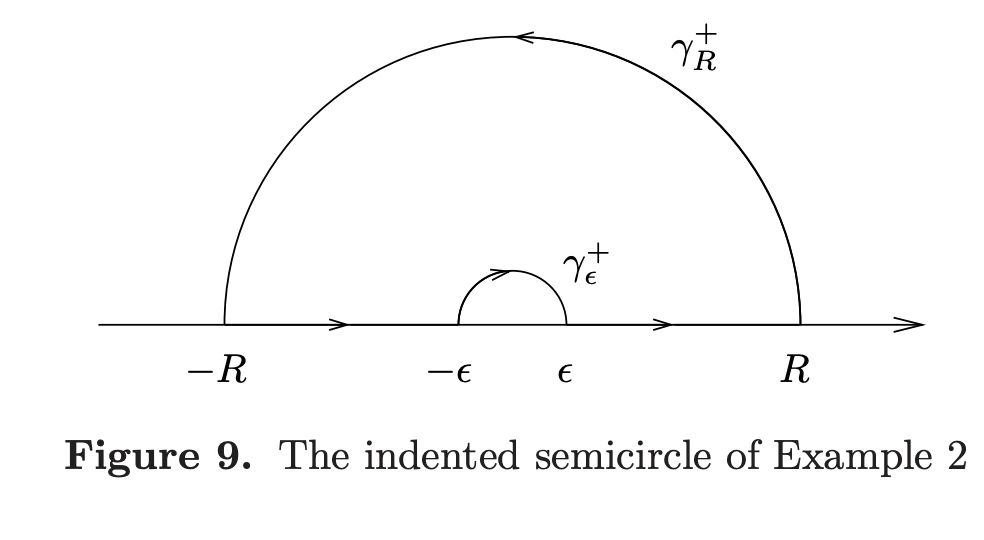
\includegraphics[scale = 0.5]{Indented_Semicircle.png}.
  \end{center}
  Take $f(z) = \frac{e^{iz}}{z}$ and we have that, by Cauchy's theorem, 
  \[
  0 = \int_{\gamma}\frac{e^{iz}}{z} = \int_{-R}^{-\epsilon} \frac{e^{ix}}{x}\mathrm{d}x + \int_{\gamma_{\epsilon}^+}\frac{e^{iz}}{z} \mathrm{d}z + \int_{\epsilon}^{R}\frac{e^{ix}}{x}\mathrm{d}x + \int_{\gamma_R^+}\frac{e^{iz}}{z}\mathrm{d}z.  
  \]
  Observe
  \begin{align*}
    \left|\int_{\gamma_R} \frac{e^{iz}}{z} \mathrm{d}z \right| &= \left|\int_0^{\pi}\frac{e^{iRe^{i \theta}}}{Re^{i \theta}}Rie^{i \theta} \mathrm{d} \theta \right|\\
    &\numleq{a} \int_0^{\pi}\left|e^{iRe^{i \theta}} \right| \mathrm{d} \theta \\ 
    &= \int_0^{\pi} \left|e^{i \cos(\theta)}\right|\left|e^{-R \sin(\theta)} \right|\mathrm{d}\theta \\
    &= \int_0^{\pi}e^{-R \sin(\theta)} \mathrm{d}\theta \\
    &\numleq{b} \int_0^{\pi}e^{-R\left(1 - \frac{2}{\pi} \left|\theta - \frac{\pi}{2}\right|\right)}\mathrm{d}\theta \\
    &= e^{-R}\int_0^{\pi}e^{\frac{2R}{\pi}\left|\theta - \frac{\pi}{2}\right|} \mathrm{d}\theta \\
    &= e^{-R}\left(\int_0^{\frac{\pi}{2}}e^{-\frac{2R}{\pi}\left(\theta - \frac{\pi}{2}\right)} \mathrm{d}\theta + \int_{\frac{\pi}{2}}^{\pi}e^{\frac{2R}{\pi}\left(\theta - \frac{\pi}{2}\right)} \mathrm{d}\theta \right) \\
    &= \int_0^{\frac{\pi}{2}}e^{-\frac{2R}{\pi}\theta} \mathrm{d} \theta + e^{-2R} \int_{\frac{\pi}{2}}^{\pi}e^{\frac{2R}{\pi}\theta}\mathrm{d}\theta \\
    &\numeq{c}\left[-\frac{\pi e^{-\frac{2R}{\pi}\theta}}{2R} \right]_0^{\frac{\pi}{2}} + e^{-2R}\left[\frac{\pi e^{\frac{2R}{\pi}\theta}}{2R} \right]_{\frac{\pi}{2}}^{\pi} \\
    &= -\frac{\pi e^{-R}}{2R} + \frac{\pi}{2R} + \frac{\pi}{2R} - \frac{\pi e^{-R}}{2R} \xrightarrow[R \to \infty]{} 0
  \end{align*}
  with steps $(a)-(c)$ justified as thus:
  \begin{enumerate}[\indent(a)]
   \item Triangle inequality for integrals
   \item hint provided in homework that $\sin \theta \geq 1 - \frac{2}{\pi}\left|\theta -\frac{\pi}{2}\right|$ for $\theta \in \left[0, \frac{\pi}{2} \right]$
   \item real-valued integral so we can use known integral tricks to solve. 
  \end{enumerate}
  We will now tackle the integral $\int_{\gamma_{\epsilon}}\frac{e^{iz}}{z} \mathrm{d}z$. In class, we were given a lemma that states since $f$ is continuous on an open disk around the indented semicircle with $0 \leq arg(z) \leq \pi$, and $\lim\limits_{z \to 0}z f(z) = 1$, then we have that 
  \[
  \lim\limits_{\epsilon \to 0^+} \int_{\gamma_{\epsilon}}f(z) \mathrm{d}z = i(0 - \pi) = -i \pi  
  \] 
  as the curve travels from $\theta = \pi$ to $ \theta = 0$.
  Rearranging the equation, we get that 
  \[
    \int_{-R}^{-\epsilon} \frac{e^{ix}}{x}\mathrm{d}x + \int_{\epsilon}^{R}\frac{e^{ix}}{x}\mathrm{d}x  =  -\int_{\gamma_{\epsilon}^+}\frac{e^{iz}}{z} \mathrm{d}z - \int_{\gamma_R^+}\frac{e^{iz}}{z}\mathrm{d}z.
  \]
  Taking $\epsilon \to 0$ and $R \to \infty$ see 
  \[
  \lim\limits_{\epsilon \to 0, R \to \infty} \left(\int_{-R}^{-\epsilon} \frac{e^{ix}}{x}\mathrm{d}x + \int_{\epsilon}^{R}\frac{e^{ix}}{x}\mathrm{d}x \right) =\lim\limits_{\epsilon \to 0, R \to \infty} \left(  -\int_{\gamma_{\epsilon}^+}\frac{e^{iz}}{z} \mathrm{d}z - \int_{\gamma_R^+}\frac{e^{iz}}{z}\mathrm{d}z \right) 
  \]
  implies
\[
  \int_{-\infty}^{\infty} \frac{e^{ix}}{x} \mathrm{d}x = i \pi. 
\]
We now decompose to our desired integral
\begin{align*}
  i \pi &= \int_{-\infty}^{\infty} \frac{e^{ix}}{x} \mathrm{d}x \\
  &= \int_{-\infty}^{\infty} \frac{\cos(x) + i\sin(x)}{x} \mathrm{d}x \\
  &= \int_{-\infty}^{\infty} \frac{\cos(x)}{x} \mathrm{d}x + i\int_{-\infty}^{\infty} \frac{\sin(x)}{x}\mathrm{d}x.
\end{align*} 
Looking at only the imaginary part, it can be seen that we must then have 
\[
 \int_{-\infty}^{\infty} \frac{cos(x)}{x}\mathrm{d}x = 0 
\]
and thus, we have that 
\[
 \pi = \int_{-\infty}^{\infty} \frac{\sin(x)}{x}\mathrm{d}x 
\]
and using the fact that $\frac{\sin(x)}{x}$ is even we get the desired result
\[
 \frac{\pi}{2} = \int_0^{\infty}\frac{\sin(x)}{x} \mathrm{d}x
\]

\end{proof}

\section*{3.}
\begin{proof}
  Let $A = \sqrt{a^2 + b^2}$, $\cos(\omega) = \frac{a}{A}$ which implies $\sin(\omega) = \frac{b}{A}$. Note, that we must take a sector where $a > 0$ always, so we must have that $\omega \in \left[0, \frac{\pi}{2}\right)$ making our sector look like the image below:

\begin{center}
\tikzset{every picture/.style={line width=0.75pt}} %set default line width to 0.75pt        

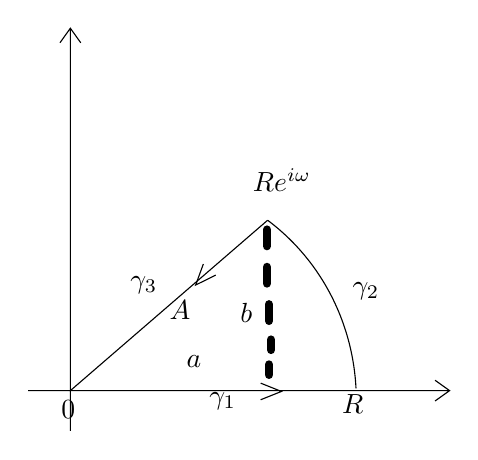
\begin{tikzpicture}[x=0.75pt,y=0.75pt,yscale=-1,xscale=1]
%uncomment if require: \path (0,300); %set diagram left start at 0, and has height of 300

%Shape: Axis 2D [id:dp7523876561837348] 
\draw  (236,225.6) -- (439,225.6)(256.3,51) -- (256.3,245) (432,220.6) -- (439,225.6) -- (432,230.6) (251.3,58) -- (256.3,51) -- (261.3,58)  ;
%Shape: Arc [id:dp5531989103320447] 
\draw  [draw opacity=0] (351.34,143.51) .. controls (377.42,163.05) and (392.33,193.04) .. (393.92,224.52) -- (285.23,232.56) -- cycle ; \draw   (351.34,143.51) .. controls (377.42,163.05) and (392.33,193.04) .. (393.92,224.52) ;  
%Straight Lines [id:da06183978011979585] 
\draw    (351.34,143.51) -- (256.3,225.6) ;
\draw   (348,222) -- (358,226) -- (348,230) ;
\draw   (326.32,169.96) -- (316.66,174.72) -- (320.37,164.61) ;
%Shape: Free Drawing [id:dp5340330195882352] 
\draw  [line width=3] [line join = round][line cap = round] (351,148) .. controls (351,150.67) and (351,153.33) .. (351,156) ;
%Shape: Free Drawing [id:dp8486705622564401] 
\draw  [line width=3] [line join = round][line cap = round] (351,166) .. controls (351,168.67) and (351,171.33) .. (351,174) ;
%Shape: Free Drawing [id:dp14425627538467234] 
\draw  [line width=3] [line join = round][line cap = round] (352,184) .. controls (352,186.67) and (352,189.33) .. (352,192) ;
%Shape: Free Drawing [id:dp2865369776568436] 
\draw  [line width=3] [line join = round][line cap = round] (353,201) .. controls (353,202.67) and (353,204.33) .. (353,206) ;
%Shape: Free Drawing [id:dp4486095535590433] 
\draw  [line width=3] [line join = round][line cap = round] (352,213) .. controls (352,214.67) and (352,216.33) .. (352,218) ;

% Text Node
\draw (343,117.4) node [anchor=north west][inner sep=0.75pt]    {$Re^{i\omega }$};
% Text Node
\draw (386,226.4) node [anchor=north west][inner sep=0.75pt]    {$R$};
% Text Node
\draw (244,226.4) node [anchor=north west][inner sep=0.75pt]    {$ \begin{array}{l}
0\\
\end{array}$};
% Text Node
\draw (284,169.4) node [anchor=north west][inner sep=0.75pt]    {$\gamma _{3}$};
% Text Node
\draw (391,172.4) node [anchor=north west][inner sep=0.75pt]    {$\gamma _{2}$};
% Text Node
\draw (322,225.4) node [anchor=north west][inner sep=0.75pt]    {$\gamma _{1}$};
% Text Node
\draw (311,207.4) node [anchor=north west][inner sep=0.75pt]    {$a$};
% Text Node
\draw (337,182.4) node [anchor=north west][inner sep=0.75pt]    {$b$};
% Text Node
\draw (302.82,180.96) node [anchor=north west][inner sep=0.75pt]    {$A$};


\end{tikzpicture}
\end{center}
By Cauchy's theorem, we have that 
\begin{align*}
 0 &= \int_{\gamma}e^{-Az} \mathrm{d}z \\
 &= \int_{\gamma_1} e^{-Az} \mathrm{d}z + \int_{\gamma_2}e^{-Az} \mathrm{d}z + \int_{\gamma_3} e^{-Az} \mathrm{d}z \\
 &\numeq{a} \int_0^R e^{-Ax} \mathrm{d}x + \int_0^{\omega}e^{-ARe^{i \theta}} i Re^{i \theta} \mathrm{d}\theta - \int_0^R e^{-Axe^{i \omega}} e^{i \omega}\mathrm{d}x  
\end{align*}
where step $(a)$ is justfied using the fact that $\int_{\gamma} f(z) \mathrm{d}z = \int_a^b f(z(t))z'(t) \mathrm{d}t$. We begin by looking at the integral over $\gamma_2$:
\begin{align*}
  \left|\int_0^{\omega}e^{-ARe^{i \theta}} iRe^{i \theta} \mathrm{d} \theta\right| &\numleq{a} \int_0^{\omega}\left|e^{-ARe^{i \theta}} iRe^{i \theta} \right| \mathrm{d} \theta \\
  &= R \int_0^{\omega} e^{-AR \cos(\theta)} \mathrm{d}\theta \\
  &\numleq{b}R\int_0^{\omega}e^{-AR\left(1 - \frac{2}{\pi}\theta \right)} \mathrm{d}\theta \\
  &= Re^{-AR}\int_0^{\omega}e^{\frac{2}{\pi}AR\theta} \mathrm{d} \theta \\
  &\numeq{c} Re^{-AR} \left[\frac{\pi}{2AR}e^{\frac{2}{\pi}AR\theta}\right]_0^{\omega} \\
  &= \frac{\pi e^{AR\left(\frac{2}{\pi}\omega - 1 \right)}}{2A} - \frac{\pi e^{-AR}}{2A}
\end{align*}  
with steps $(a)-(c)$ justified:
\begin{enumerate}[\indent(a)]
 \item Triangle inequality for integrals
 \item Inequality given in the hint for the homework that $\cos \theta \geq 1 - \frac{2}{\pi}\theta$ for $\theta \in \left[0, \frac{\pi}{2} \right]$
 \item Real-valued integral can be solved with usual techniques. 
\end{enumerate}
Notice now that since $\omega \in \left[0, \frac{\pi}{2} \right)$ that we will always have that $AR \left(\frac{2}{\omega} - 1 \right) < 0$ as $A, R > 0$. Therefore, we must have 
\[
 \lim\limits_{R \to \infty} \frac{\pi e^{AR\left(\frac{2}{\pi}\omega - 1 \right)}}{2A} - \frac{\pi e^{-AR}}{2A} = 0.
\]
Analyzing the integral over $\gamma_2$, we can quickly see that
\begin{align*}
  \int_0^{R} e^{-Ax} \mathrm{d}x &= -\frac{1}{A}\left[e^{-Ax} \right]_0^R \\
  &= -\frac{1}{A} \left(e^{-AR} - 1 \right) \xrightarrow[R \to \infty]{} \frac{1}{A}.
\end{align*}
Lastly, we take a look at the integral over $\gamma_3$:
\begin{align*}
  \int_0^R e^{-Axe^{i \omega}}e^{i \omega} \mathrm{d}x &= e^{i \omega}\int_0^Re^{-Ax (\cos(\omega) + i \sin(\omega))} \mathrm{d}x \\
  &\numeq{a}e^{i \omega}\int_0^Re^{-Ax \frac{a}{A}}e^{-iAx\frac{b}{A}}\mathrm{d}x \\
  &= (\cos(\omega) + i \sin(\omega)) \int_0^Re^{-xa}(\cos(bx) -i\sin(bx))\mathrm{d}x \\
  &\numeq{b}\left(\frac{a}{A} +i\frac{b}{A}\right) \left(\int_0^Re^{-xa}\cos(bx) \mathrm{d}x -i \int_0^R e^{-xa}\sin(bx) \mathrm{d}x \right). 
\end{align*}
Steps $(a)-(b)$ are both justfied by that $\cos(\omega) = \frac{a}{A}$ and $\sin(\omega) = \frac{b}{A}$. Stitching everything back together and taking the limit of $R \to \infty$, we ascertain
\[
 0 = \frac{1}{A} -  \left(\frac{a}{A} +i\frac{b}{A}\right) \left(\int_0^Re^{-xa}\cos(bx) \mathrm{d}x -i \int_0^R e^{-xa}\sin(bx) \mathrm{d}x \right)
\]
which implies
\[
 \frac{1}{A} = \left(\frac{a}{A} +i\frac{b}{A}\right) \left(\int_0^Re^{-xa}\cos(bx) \mathrm{d}x -i \int_0^R e^{-xa}\sin(bx) \mathrm{d}x \right). 
\]
Multiplying each side by the complex conjugate of $\frac{a}{A} +i\frac{b}{A}$ we get
\[
 \left(\frac{a}{A} - i \frac{b}{A} \right)\frac{a}{A} = \int_0^Re^{-xa}\cos(bx) \mathrm{d}x -i \int_0^R e^{-xa}\sin(bx) \mathrm{d}x
\]
and thus 
\[
 \frac{a}{a^2+b^2} -i\frac{b}{a^2 + b^2} = \int_0^Re^{-xa}\cos(bx) \mathrm{d}x -i \int_0^R e^{-xa}\sin(bx) \mathrm{d}x. 
\]
Looking at the real and imaginary parts, we see
\[
  \frac{a}{a^2+b^2} = \int_0^Re^{-xa}\cos(bx) \mathrm{d}x \text{   and  } \frac{b}{a^2 + b^2} = \int_0^Re^{-xa}\sin(bx) \mathrm{d}x. 
\]
\end{proof}

\section*{5.}
\begin{proof}
  Suppose $f$ is continuously complex differentiable on $\Omega$, and $T \subset \Omega$ is a triangle whose interior is also contained in $\Omega$. Denote $F$ and $G$ as the real and imaginary parts of $f$, respectively. Recall that for a complex-valued function to be continuously differentiable, both the real and imaginary parts of the function must be continuously differentiable. Let $z(t):[a, b] \to T$ be a parametrization of the triangle with $z = x + iy$.  Therefore, 
  \begin{align*}
    \int_T f(z) \mathrm{d}z &= \int_a^b f(z(t)) z'(t) \mathrm{d}t\\ 
    &= \int_a^b f(z(t)) \left(\frac{\partial x}{\partial t} +i \frac{\partial y}{\partial t} \right) \mathrm{d}t\\
    &= \int_a^b f(z(t)) \left(\frac{\partial x}{\partial t} +i \frac{\partial y}{\partial t} \right) \mathrm{d}t\\
    &= \int_a^b (F(z(t)) +iG(z(t))) \left(\frac{\partial x}{\partial t} +i \frac{\partial y}{\partial t} \right) \mathrm{d}t\\ 
    &\numeq{a} \int_a^b F(z(t))\mathrm{d}x + iF(z(t)) \mathrm{d}y + iG(z(t)) \mathrm{d}x -G(z(t)) \mathrm{d}y\\
    &= \int_a^bF(z) \mathrm{d}x - G(z) \mathrm{d}y + i\int_a^b F(z) \mathrm{d}y + G(z) \mathrm{d}x \\
    &= \int_T F \mathrm{d}x - G \mathrm{d}y + i\int_T F \mathrm{d}y + G\mathrm{d}x\\
     &\numeq{b} \int_{\text{Interior of }T} \left(\frac{\partial G}{\partial x} + \frac{\partial F}{ \partial y} \right) \mathrm{d}x\mathrm{d}y + \int_{\text{Interior of }T} \left(\frac{\partial F}{\partial x}- \frac{\partial G}{\partial y} \right) \mathrm{d}x\mathrm{d}y
  \end{align*}
  where step $(a)-(b)$ are justified:
  \begin{enumerate}[\indent(a)] 
    \item $\frac{\partial x}{\partial t} dt = dx$, $\frac{\partial y}{\partial t} dt = dy$
    \item Green's theorem. 
  \end{enumerate} 
  By the Cauchy-Riemann equations, we have that 
  \[
  \frac{\partial F}{\partial y} = -\frac{\partial G}{\partial x} , \ \frac{\partial F}{ \partial x} = \frac{\partial G}{ \partial y}
  \]
  and thus 
  \[
    \int_{\text{Interior of }T} \left(\frac{\partial G}{\partial x} + \frac{\partial F}{ \partial y} \right) \mathrm{d}x\mathrm{d}y + \int_{\text{Interior of }T} \left(\frac{\partial F}{\partial x}- \frac{\partial G}{\partial y} \right) \mathrm{d}x \mathrm{d}y = 0. 
  \]


\end{proof}












\end{document}














